\documentclass{scrartcl}
 
\usepackage[utf8]{inputenc}
\usepackage[T1]{fontenc}
\usepackage{lmodern}
\usepackage{listings}
\usepackage[english]{cleveref}
\usepackage[english]{babel}
\usepackage{graphicx}

\lstdefinelanguage{scala}{
  morekeywords={abstract,case,catch,class,def,%
    do,else,extends,false,final,finally,%
    for,if,implicit,import,match,mixin,%
    new,null,object,override,package,%
    private,protected,requires,return,sealed,%
    super,this,throw,trait,true,try,%
    type,val,var,while,with,yield},
  otherkeywords={=>,<-,<\%,<:,>:,\#,@},
  sensitive=true,
  morecomment=[l]{//},
  morecomment=[n]{/*}{*/},
  morestring=[b]",
  morestring=[b]',
  morestring=[b]"""
}

\lstset{
  language=scala,
  basicstyle=\scriptsize,
  numberstyle=\scriptsize,
  frame=L,
  captionpos=b,
  tabsize=4,
  numbers=left,
  stepnumber=5,
  firstnumber=1
}

\title{ReSwing -- A Reactive Interface for Scala Swing}
\author{}
\date{}
\begin{document}

\maketitle
\section{Basic Design Overview -- Java Swing\,/\,Scala Swing\,/\,ReSwing}
\label{sec:overview}
The Scala Swing library is implemented as a wrapper around the Java Swing library. It mirrors the Java Swing class hierarchy and every component holds a reference to the underlying Java Swing component. Building on Scala Swing, the ReSwing library adds another layer to this architecture. It provides its own class hierarchy containing all reactively enabled components. \Cref{fig:overview} shows a small, representative part of these class hierarchies.

\begin{figure}[h]
  \centering
  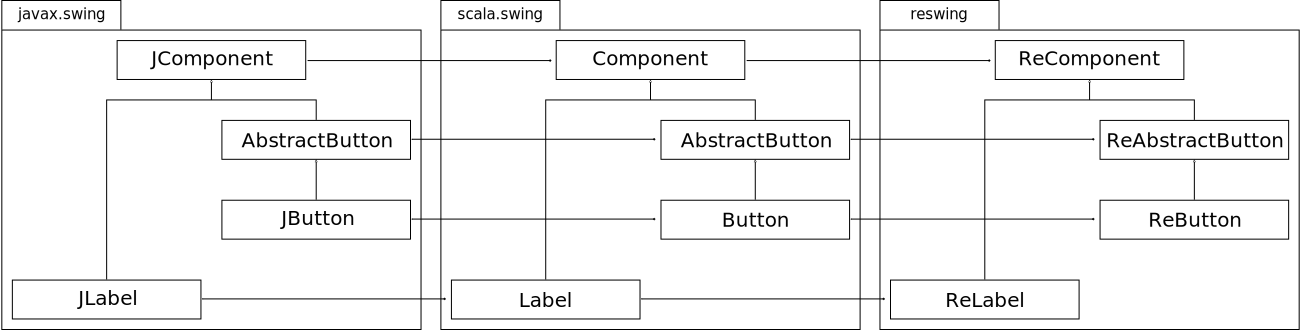
\includegraphics[width=\textwidth]{overview}
  \caption{Scala Swing and ReSwing wrapper architecture}
  \label{fig:overview}
\end{figure}

The purpose of the ReSwing library is to provide reactive values for certain Swing properties. Since it is possible to define a signal for these values and signals are defined once the signal is created and are not re-assignable, properties in the ReSwing library are passed to the components' constructors and cannot be assigned later. This also results in a slightly different approach when constructing ReSwing components as shown in \cref{lst:scala-swing-example} and \cref{lst:reswing-example}.

\hspace{1em}\begin{lstlisting}[caption={Example for a Label component instantiation in Scala Swing},label={lst:scala-swing-example}]
val label = new Label
label.text = "foobar"
label.preferredSize = new Dimension(400, 40)
\end{lstlisting}

\begin{lstlisting}[caption={Example for a ReLabel component instantiation in ReSwing},label={lst:reswing-example}]
val label = new ReLabel(
    text = "foobar"
    preferredSize = new Dimension(400, 40)
)
\end{lstlisting}

\section{ReSwing Events}
\label{sec:events}
The ReSwing library provides ReScala events for Scala Swing events like, e.g., button clicks. They can be accessed and used just like any other ReScala event. Every occurrence of a Scala Swing event causes the related ReScala event of the ReSwing component to be fired.

\section{ReSwing Reactive Values}
\label{sec:reactive-values}
The ReSwing library allows the application to set reactive values and will then ensure that the underlying Swing library updates the user interface accordingly. Also, changes made by the user that are published by the Scala Swing library are reflected in the reactive values which the ReSwing library provides. So it acts as a middleware to translate between the Scala Swing getter, setter and reactor system and the ReScala signal and event system.

There are values (e.g.\ the value representing the text in a text input field) that can be changed by both the application and the user. This rises the question of how to handle two different input sources for these reactive values. The library ensures that the signals set by the application and the changes resulting from user interaction are consistently represented. This is achieved by disallowing the user to make changes in certain cases.

There are three different ways to initialize a reactive value which determine how changes to reactive values are handled:
\begin{itemize}
\item\emph{Initializing directly with the value} will set the reactive value to the given value immediately upon creation. The user can change the value afterwards.
\item\emph{Initializing with an event stream} will update the reactive value on each event occurrence. The user can change the value.
\item\emph{Initializing with a signal} ensures that the reactive value always holds the value given by the signal. Hence, the user is not allowed to change the value.
\end{itemize}

For all three cases, the respective value can just be passed to the constructor of the component as shown in \cref{lst:initializing-reactive-values}.

\hspace{1em}\begin{lstlisting}[caption={Initializing a reactive value of a ReSwing component},label={lst:initializing-reactive-values}]
val value: String
val label = new ReTextArea(
    text = value 
)

val event: Event[String]
val label = new ReTextArea(
    text = event
)

val signal: Signal[String] 
val label = new ReTextArea( 
    text = signal 
)
\end{lstlisting}

After a component instance has been constructed, all reactive values can be treated as signals when accessing the properties (e.g.\ \texttt{Signal \{ label.text() \}}).

\section{Extending the ReSwing Library -- Defining Reactive Values}
\label{sec:defining-reactive-values}
The library offers a declarative syntax to define which reactive value should map to which property of the underlying Swing component. Using this syntax ensures that value changes are properly propagated from the ReSwing library to the Scala Swing library and vice versa.

For a reactive property, you need to specify:
\begin{itemize}
\item the \emph{getter} of the underlying Swing property to retrieve the value
\item the \emph{setter} of the underlying Swing property to set the value (if the reactive property can be changed by the application)
\item a way to identify changes of the underlying Swing property, either by giving the bound property name or a Scala Swing event type
\end{itemize}
Additionally it is possible to force other properties to hold a specified value, if the reactive value should not be changeable by the user. This can be the case if the reactive value is initialized with a signal as described in \cref{sec:reactive-values}.

Examples of some reactive values defined in different ways are given in \cref{lst:defining-reactive-values}.

\hspace{1em}\begin{lstlisting}[caption={Defining Reactive Values},label={lst:defining-reactive-values}]
class ReLabel(val text: ReSwingValue[String] = ()) extends ReComponent {
  text using (peer.text _, peer.text_= _, "text")
}

class ReTextComponent(val text: ReSwingValue[String] = ()) extends ReComponent {
  (text using (peer.text _, peer.text_= _, classOf[ValueChanged])
        force ("editable", peer.editable_= _, false))
}

abstract class ReComponent extends ReUIElement {
  val hasFocus = ReSwingValue using (peer.hasFocus _, classOf[FocusGained],
                                                      classOf[FocusLost])
}
\end{lstlisting}

\end{document}
